\documentclass{article}
\usepackage[utf8]{inputenc}
\usepackage{multicol}
\usepackage{listings}
\usepackage{amssymb}
\usepackage{enumitem}
\usepackage{graphicx}
\usepackage{amsthm}
\usepackage{hyperref}
\usepackage[ruled,vlined]{algorithm2e}
\usepackage{tikz}
\usetikzlibrary{arrows}
\newtheorem{theorem}{Theorem}
\newtheorem{definition}{Definition}

\SetKwProg{Fn}{Function}{}{}
\SetKwProg{Proc}{Procedure}{}{}
\SetKwFunction{isBalanced}{isBalanced}
\SetKwFunction{checkBalance}{checkBalance}

%=====================================
%			Assignment 7
%=====================================

\begin{document}

\title{Weekly Assignment 7}
\author{Tony Lopar s1013792}
\date{19th October 2017}
\maketitle

\paragraph{Deadline:} 25th October 2017, 6pm.
\paragraph{Solutions:} The solutions can be found below the exercises.

\section*{Exercise 1. \textit{Weight: 10\%}}
How many BST can you build with the following elements:$\{3, 5, 8, 12\}$? Draw them.

\subsection*{Solutions 1}
There are 15 different BST's possible. All these options are drawn below.
\begin{center}
\begin{multicols}{5}
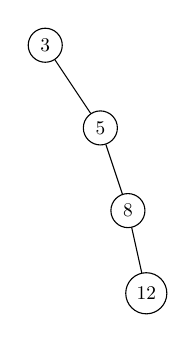
\begin{tikzpicture}[-, level/.style={sibling distance = 2cm/#1, level distance = 1.5cm}, scale=0.7,transform shape]
  \node[circle,draw](z){$3$}
      child[missing]
      child{
          node[circle,draw]{5}
          child[missing]
          child{
              node[circle,draw]{8}
              child[missing]
              child{
                  node[circle,draw]{12}
              }
          }
      };
\end{tikzpicture}
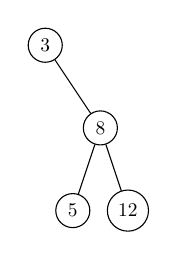
\begin{tikzpicture}[-, level/.style={sibling distance = 2cm/#1, level distance = 1.5cm}, scale=0.7,transform shape]
  \node[circle,draw](z){$3$}
      child[missing]
      child{
          node[circle,draw]{8}
          child{
              node[circle,draw]{5}
          }
          child{
              node[circle,draw]{12}
          }
      };
\end{tikzpicture}
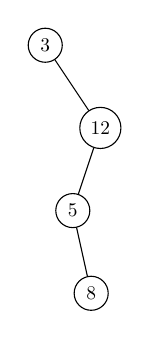
\begin{tikzpicture}[-, level/.style={sibling distance = 2cm/#1, level distance = 1.5cm}, scale=0.7,transform shape]
  \node[circle,draw](z){$3$}
      child[missing]
      child{
          node[circle,draw]{12}
          child{
              node[circle,draw]{5}
              child[missing]
              child{
                  node[circle,draw]{8}
              }
          }
          child[missing]
      };
\end{tikzpicture}
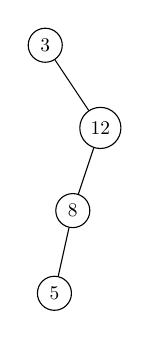
\begin{tikzpicture}[-, level/.style={sibling distance = 2cm/#1, level distance = 1.5cm}, scale=0.7,transform shape]
  \node[circle,draw](z){$3$}
      child[missing]
      child{
          node[circle,draw]{12}
          child{
              node[circle,draw]{8}
              child{
                  node[circle,draw]{5}
              }
              child[missing]
          }
          child[missing]
      };
\end{tikzpicture}
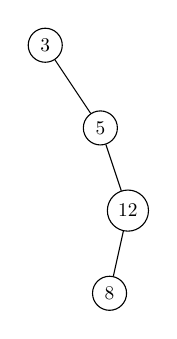
\begin{tikzpicture}[-, level/.style={sibling distance = 2cm/#1, level distance = 1.5cm}, scale=0.7,transform shape]
  \node[circle,draw](z){$3$}
      child[missing]
      child{
          node[circle,draw]{5}
          child[missing]
          child{
              node[circle,draw]{12}
              child{
                  node[circle,draw]{8}
              }
              child[missing]
          }
      };
\end{tikzpicture}

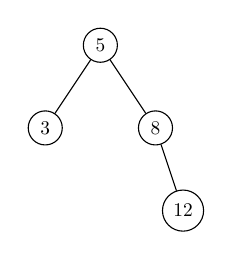
\begin{tikzpicture}[-, level/.style={sibling distance = 2cm/#1, level distance = 1.5cm}, scale=0.7,transform shape]
  \node[circle,draw](z){$5$}
      child{
        node[circle,draw]{3}
      }
      child{
          node[circle,draw]{8}
          child[missing]
          child{
              node[circle,draw]{12}
          }
      };
\end{tikzpicture}
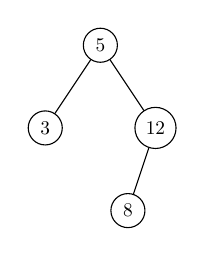
\begin{tikzpicture}[-, level/.style={sibling distance = 2cm/#1, level distance = 1.5cm}, scale=0.7,transform shape]
  \node[circle,draw](z){$5$}
      child{
        node[circle,draw]{3}
      }
      child{
          node[circle,draw]{12}
          child{
              node[circle,draw]{8}
          }
          child[missing]
      };
\end{tikzpicture}

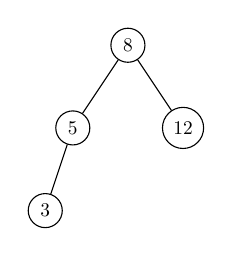
\begin{tikzpicture}[-, level/.style={sibling distance = 2cm/#1, level distance = 1.5cm}, scale=0.7,transform shape]
  \node[circle,draw](z){$8$}
      child{
        node[circle,draw]{5}
        child{
            node[circle,draw]{3}
        }
        child[missing]
      }
      child{
          node[circle,draw]{12}
      };
\end{tikzpicture}
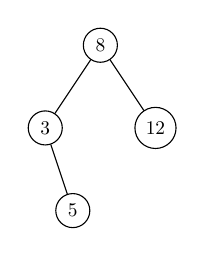
\begin{tikzpicture}[-, level/.style={sibling distance = 2cm/#1, level distance = 1.5cm}, scale=0.7,transform shape]
  \node[circle,draw](z){$8$}
      child{
        node[circle,draw]{3}
        child[missing]
        child{
            node[circle,draw]{5}
        }
      }
      child{
          node[circle,draw]{12}
      };
\end{tikzpicture}

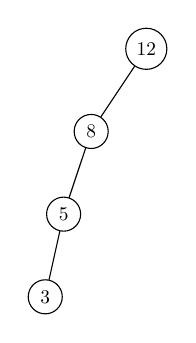
\begin{tikzpicture}[-, level/.style={sibling distance = 2cm/#1, level distance = 1.5cm}, scale=0.7,transform shape]
  \node[circle,draw](z){$12$}
      child{
          node[circle,draw]{8}
          child{
              node[circle,draw]{5}
              child{
                  node[circle,draw]{3}
              }
              child[missing]
          }
          child[missing]
      }
      child[missing];
\end{tikzpicture}
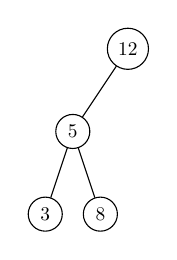
\begin{tikzpicture}[-, level/.style={sibling distance = 2cm/#1, level distance = 1.5cm}, scale=0.7,transform shape]
  \node[circle,draw](z){$12$}
      child{
          node[circle,draw]{5}
          child{
              node[circle,draw]{3}
          }
          child{
              node[circle,draw]{8}
          }
      }
      child[missing];
\end{tikzpicture}
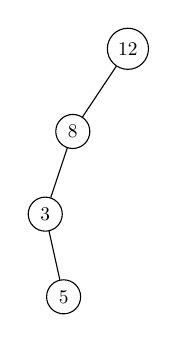
\begin{tikzpicture}[-, level/.style={sibling distance = 2cm/#1, level distance = 1.5cm}, scale=0.7,transform shape]
  \node[circle,draw](z){$12$}
      child{
          node[circle,draw]{8}
          child{
              node[circle,draw]{3}
              child[missing]
              child{
                  node[circle,draw]{5}
              }
          }
          child[missing]
      }
      child[missing];
\end{tikzpicture}
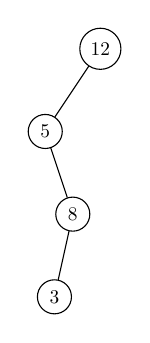
\begin{tikzpicture}[-, level/.style={sibling distance = 2cm/#1, level distance = 1.5cm}, scale=0.7,transform shape]
  \node[circle,draw](z){$12$}
      child{
          node[circle,draw]{5}
          child[missing]
          child{
              node[circle,draw]{8}
              child{
                  node[circle,draw]{3}
              }
              child[missing]
          }
      }
      child[missing];
\end{tikzpicture}
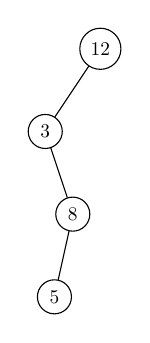
\begin{tikzpicture}[-, level/.style={sibling distance = 2cm/#1, level distance = 1.5cm}, scale=0.7,transform shape]
  \node[circle,draw](z){$12$}
      child{
          node[circle,draw]{3}
          child[missing]
          child{
              node[circle,draw]{8}
              child{
                  node[circle,draw]{5}
              }
              child[missing]
          }
      }
      child[missing];
\end{tikzpicture}
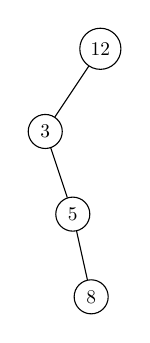
\begin{tikzpicture}[-, level/.style={sibling distance = 2cm/#1, level distance = 1.5cm}, scale=0.7,transform shape]
  \node[circle,draw](z){$12$}
      child{
          node[circle,draw]{3}
          child[missing]
          child{
              node[circle,draw]{5}
              child[missing]
              child{
                  node[circle,draw]{8}
              }
          }
      }
      child[missing];
\end{tikzpicture}
\end{multicols}
\end{center}
\newpage
\section*{Exercise 2. \textit{Weight: 20\%}}
Let us consider all the integers between 1 and $2^n - 1$ for a given $n$. Give
\begin{enumerate}
  \item one insertion order of these integers maximizing height.
  \item one insertion order of these integers minimizing height (also giving a balanced BST).
\end{enumerate}

\subsection*{Solutions 2}
\begin{enumerate}
  \item Inserting all the elements in an ascending or descending order.
  \item Inserting the median of the list as root. Then take on the left the median of the elements lower than the root and on the right the median of the elements greater than the root. This should be repeated until we have only one value left on both sides of the median.
  \newline
  For example, if we take $n = 3$, then we have the integers 1 until 7. The median here is 4 which will be the root. The median of the lower values is 2 which will be the left child of the root. On the right side we have 6 as median. Since both median only have one integer on both sides, we will insert these as children. The tree will be as follows:
  \begin{center}
  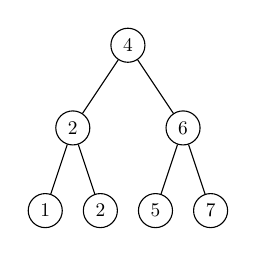
\begin{tikzpicture}[-, level/.style={sibling distance = 2cm/#1, level distance = 1.5cm}, scale=0.7,transform shape]
    \node[circle,draw](z){$4$}
        child{
            node[circle,draw]{2}
            child{
                node[circle,draw]{1}
            }
            child{
                node[circle,draw]{2}
            }
        }
        child{
            node[circle,draw]{6}
            child{
                node[circle,draw]{5}
            }
            child{
                node[circle,draw]{7}
            }
        };
  \end{tikzpicture}
\end{center}
\end{enumerate}

\newpage
\section*{Exercise 3. \textit{Weight: 20\%}}
Write an algorithm running in $\mathcal{O}(n)$ time and returning whether a binary tree is balanced or not.

\subsection*{Solutions 3}
This algorithm should check whether the height of both subtrees has a maximum height difference of 1. This should be done for every subtree. We could achieve this recursively. We should first check the height of the childs of the root, but in order to discover the height we have to find out the distance to the leaves.

\begin{algorithm}[h!]
  \DontPrintSemicolon
    \Proc{\checkBalance{Node root}}{
    $result \leftarrow isBalanced(root)$ \;
        \If{$result > 0$} {
      \KwRet{true} \;
    }
    \Else{
      \KwRet{false} \;
    }
    }
    \Proc{\isBalanced{Node node}}{
      \If{$node = nil$}{
        \KwRet{0} \;
      }
      $leftH \leftarrow isBalanced(node.left)$ \;
      \If{$leftH = -1$} {
        \KwRet{-1} \;
      }
      $rightH \leftarrow isBalanced(node.right)$ \;
      \If{$rightH = -1$} {
        \KwRet{-1} \;
      }
      $diff \leftarrow leftH-rightH$ \;
      \If{$|diff| > 1$} {
        \KwRet{-1} \;
      }
      \If{$leftH < rightH$}{
        \KwRet{$1 + rightH$} \;
      } \Else{
        \KwRet{$1 + leftH$} \;
      }
    }
    \caption{Check whether tree is balanced}
\end{algorithm}

\newpage
\section*{Exercise 4. \textit{Weight: 20\%}}
We consider in this exercise that the depth of the root of a BST is 0.
\begin{enumerate}
  \item Compute the maximal number of nodes of a BST of depth $h$.
  \item Deduce that a BST with $n$ nodes has a depth of at least $\lceil lg(n+1) \rceil - 1$.
  \item Show by induction over $h$ that the mean depth of nodes in a full BST (that is to say, links are completely filled) of depth $h$ is comprised between $h-1$ and $h$.
\end{enumerate}

\subsection*{Solutions 4}
\begin{enumerate}
  \item The formula for computing the maximal number of nodes on depth h is $2^h$. This is the case, because every depth can have twice as much nodes as the previous one. Thus, the number of maximum nodes is growing exponential. This formula also holds for the root, because $2^0 = 1$.
  \item In order to calculate whether the formula is correct, we may verify whether this holds for a full tree and a tree with only one leave. If this follows, we may assume that this also holds for an intermediate number of leaves. Let's for example take a full tree with height 8. In this case $n = (2 \cdot 2^8 - 1) = 511$. So, by calculating $\lceil lg(511+1) \rceil - 1 = 6$ which holds because $8 > 6$.

  If we add one node to the previous example, then we have a tree with a depth of 9 that has only one leave. The value there will be $\lceil lg(512+1) \rceil - 1 = 6$ which holds because $9 > 6$.
  \item The mean depth will be in a full BST close to the leaves, since these form more than half of the nodes. Let's first try to create a formula for calculating the mean depth. In order to calculate the mean depth we have to take the sum of the deth of all nodes and divede this by the number of nodes. We already know that the number of nodes in a tree is $2^h$ + $2^h - 1$, which we can written like $2^{h + 1} - 1$ since we know that one depth higher there will be $n + 1$ nodes. In order to get the sum of the mean depths of all nodes, we have to take the sum of the number of nodes on that depth multiplied by the depth. We already computed that the maximum number of nodes on depth h is $2^h$, which is the number of nodes on that depth in a full tree. Knowing this we may use the following formula to calculate the mean depth: $\sum^{h}_{i = 1}(\frac{2^i \cdot i}{2^{h + 1} - 1})$. The initial value is set to 1, since the root has a depth of 0 which doesn't influence the sum.

  Using this formula we may calculate the mean depth of nodes. For a tree with h = 1, we will get the following sum: $\frac{2^1 \cdot 1}{2^{1 + 1} - 1} = \frac{2}{4 - 1} = \frac{2}{3}$. Since $0 < \frac{2}{3} < 1$ we have proven that this statement holds when h = 1.

  Now we have proven this for a value h, we have to prove that this also holds for h + 1 to prove it's inductive. Since at $h + 1$ there will be more nodes than in the rest of the tree. We may assume that the mean depth should be close to $h + 1$ since more than the half of the values are equal to $h + 1$.

\end{enumerate}

% mean depth = $^{\frac{1}{n}}\sum_{n5 \in V} d(5, n5)$
% full tree with height 2 has a mean depth of $\frac{2 + 2 + 2 + 2 + 1 + 1 + 0}{7} = \frac{10}{7}$. $1 < \frac{10}{7} < 2$.

\newpage
\section*{Exercise 5. \textit{Weight: 20\%}}
Each node in a binary search tree has tree attributes \emph{p}, \emph{left}, \emph{right} to store pointers.
Prove that, for each binary search tree with $n>0$ nodes, the total number of attributes with value NIL equals $n+2$.

\subsection*{Solutions 5}
In a full BST every left and right pointer is filled except in the leaves which have both pointers to NIL. The value of n in a full BST is the number of leaves $l$ and the leaves have $l - 1$ nodes above them. Since every leave has two NIL pointers, this will result in $n + 1$ NIL pointers. Besides that the root has no pointer to p, since it's the upper node of the tree. This will bring the total of nil pointers to $n + 2$.

In a non-full BST we have that there is missing at least one leave. A node above should have a NIL pointer to the position of this missing leave. Where the leave would have 2 NIL pointers, this node only has one to the position of the missing leave. This gives us one NIL pointer less when we miss a node. Since there's a node less, the sum of NIL pointers wil remain $n + 2$.

\newpage
\section*{Exercise 6. \textit{Weight: 10\%}}
How many AVL trees can you build with the following elements:$\{1, 2, 3, 4, 5\}$? Draw them.

\subsection*{Solutions 6}
We can build 6 AVL trees with these values. These are the following trees:
\begin{center}
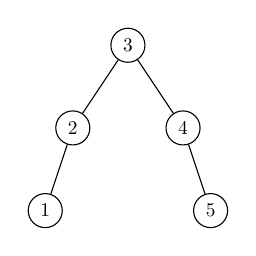
\begin{tikzpicture}[-, level/.style={sibling distance = 2cm/#1, level distance = 1.5cm}, scale=0.7,transform shape]
  \node[circle,draw](z){$3$}
      child{
        node[circle,draw]{2}
        child {
          node[circle,draw]{1}
        }
        child[missing]
      }
      child{
          node[circle,draw]{4}
          child[missing]
          child{
              node[circle,draw]{5}
          }
      };
\end{tikzpicture}
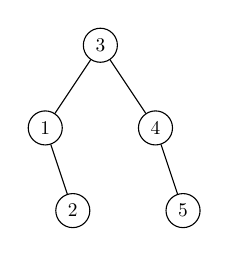
\begin{tikzpicture}[-, level/.style={sibling distance = 2cm/#1, level distance = 1.5cm}, scale=0.7,transform shape]
  \node[circle,draw](z){$3$}
      child{
        node[circle,draw]{1}
        child[missing]
        child {
          node[circle,draw]{2}
        }
      }
      child{
          node[circle,draw]{4}
          child[missing]
          child{
              node[circle,draw]{5}
          }
      };
\end{tikzpicture}
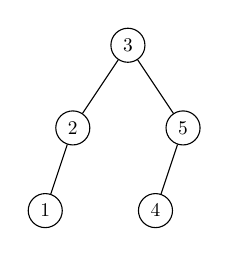
\begin{tikzpicture}[-, level/.style={sibling distance = 2cm/#1, level distance = 1.5cm}, scale=0.7,transform shape]
  \node[circle,draw](z){$3$}
      child{
        node[circle,draw]{2}
        child {
          node[circle,draw]{1}
        }
        child[missing]
      }
      child{
          node[circle,draw]{5}
          child{
              node[circle,draw]{4}
          }
          child[missing]
      };
\end{tikzpicture}
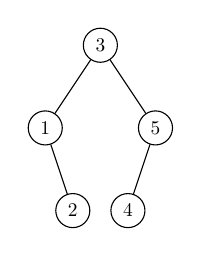
\begin{tikzpicture}[-, level/.style={sibling distance = 2cm/#1, level distance = 1.5cm}, scale=0.7,transform shape]
  \node[circle,draw](z){$3$}
      child{
        node[circle,draw]{1}
        child[missing]
        child {
          node[circle,draw]{2}
        }
      }
      child{
          node[circle,draw]{5}
          child{
              node[circle,draw]{4}
          }
          child[missing]
      };
\end{tikzpicture}

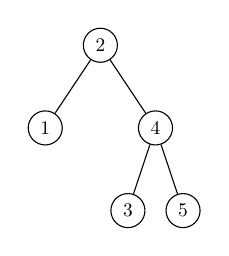
\begin{tikzpicture}[-, level/.style={sibling distance = 2cm/#1, level distance = 1.5cm}, scale=0.7,transform shape]
  \node[circle,draw](z){$2$}
      child{
        node[circle,draw]{1}
      }
      child{
          node[circle,draw]{4}
          child{
              node[circle,draw]{3}
          }
          child{
              node[circle,draw]{5}
          }
      };
\end{tikzpicture}
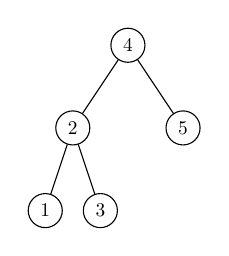
\begin{tikzpicture}[-, level/.style={sibling distance = 2cm/#1, level distance = 1.5cm}, scale=0.7,transform shape]
  \node[circle,draw](z){$4$}
      child{
        node[circle,draw]{2}
        child {
          node[circle,draw]{1}
        }
        child {
          node[circle,draw]{3}
        }
      }
      child{
          node[circle,draw]{5}
      };
\end{tikzpicture}

\end{center}

\end{document}
